\chapter{引言}
\label{cha:intro}

\section{研究背景及意义}

随着科学技术的快速发展以及工业自动化程度的日益提升,越来越多的工业设备
朝着高度集成化、复杂化、智能化的方向发展;与此同时,这些设备所处的工作
环境的复杂程度也越来越高。其中有很大一部分是用在能源、电力、交通、冶金
等国民经济支柱型产业中。比如航天器制造和发射设备、尖端数控机床、工业机
器人以及城市轨道交通设备等。我们在享受这些复杂系统给人们的生产生活带来
便利的同时,也无法忽视其背后始终存在的重大问题——故障。

近几十年来,由于这一类复杂系统突发故障而直接引发的重大事故不胜枚举。
1998年6月,德国艾雪德高速列车由于长期金属疲劳形成的微细裂缝未得到及时
发现和处理,发生车轮爆裂,导致列车脱轨,死亡人数达100多人。2011年7月23
日,甬温线特大铁路交通事故的发生导致40人死亡,172人受伤,原因是列车的
自动保护系统发生故障。航空航天领域更是事故不断。1986年美国挑战者号航天
飞机刚起飞73秒即发生解体,造成7名机组人员丧命,原因是航天飞机起飞后,
右侧火箭助推器上起密封作用的O型环失效,使原本应该密封的固体火箭助推器内
的高热高压气体泄漏。2003年哥伦比亚号航天飞机由于外储箱上的绝热材料碎片
在发射过程脱落并击中左翼前缘,损坏了热防护系统,因此在执行任务期间发生
解体,机上所有7名宇航员瞬间遇难。此外,能源化工行业也频频传来噩耗。
1986年4月发生于乌克兰的核电站反应堆爆炸事件中,当场死亡30人,泄漏强辐射
物8吨多。此外,这次核泄漏事故严重污染了附近6万多平方公里的土地,导致320
多万人遭受核辐射的侵害,可以说这是人类和平利用核能的历史上最大的灾难之一。
这些令人触目惊心的事故不断警示着我们,及早诊断出系统潜在的故障并及
时有效地进行处理,避免危险情况的发生,是保障工业系统安全稳定运行的关键
所在。目前,我们国家也非常重视这方面技术的研究和发展,在国家中长期规划、
国家自然科学基金委发展战略中都将故障诊断技术列为一个重要的发展方向。

\section{国内外研究现状}

系统在正常运行过程中,部分参数、状态或性能出现与期望不符的偏差时,我们
称系统发生了故障~\cite{van1997remarks}。通常情况下,在对系统健康状态的
监测过程中,故障诊断系统首先需要在被测对象发生故障时完成告警,其次需要
确定故障发生的类型和位置,最后需要估计出故障的严重程度。因此,一般将故
障诊断任务分解为以下三个方面:

1)故障检测(Fault Detection):确定系统是否发生故障,起到告警作用。

2)故障隔离(Fault Isolation):一旦故障检测阶段确认系统发生了故障,那
么需要进一步对故障的类型以及发生的位置进行确定。从而为维修过程提供辅助
信息,极大地提升系统设备的维修效率。

3)故障识别(Fault Identification):在完成故障隔离后,对故障的严重程度
进行估计,从而为采取何种维修手段提供重要的依据。

总体上,可以将现有的故障诊断方法分为两类:传统的基于模型的方法以及近些
年来兴起的数据驱动的方法。

基于模型的故障诊断方法的基本思想是建立系统内部结构、行为或功能的数学模
型,并且基于此模型来预测系统的行为,然后将这些模型预测值与系统的观测值
进行比较~\cite{console1999model, davis1988model, mosterman1998comprehensive}。
如果预测值与观测值一致,说明系统正常;如果存在差异,那么利用这些差异去
搜索那些能够使模型预测值与系统观测值一致的各种可能的状态假设,这些状态
假设就是基于模型的故障诊断方法得出的诊断结果~\cite{wotawa2000debugging, friedrich1999model}。

在基于模型的故障诊断方法中,系统的模型是已知的,与之不同的是,数据驱动的
故障诊断方法仅仅取决于从系统中测量的数据。 由于计算机和信息技术的快速发
展,大量的测量数据可用于提取与系统当前状态相关的有用信息,并且对决策单元
做出更好的控制和优化方案提供支持~\cite{yin2012comparison}。因此,近些年来,
无论是在研究领域还是实际工业应用中,数据驱动的故障诊断方法都受到越来越多
的重视。本文根据故障诊断模型在训练和预测过程中是否能够有效利用输入数据在
多个尺度上的特征,将数据驱动的故障诊断方法划分为单一尺度的故障诊断方法和
多尺度的故障诊断方法。如图~\ref{fig:method_summary}所示。
\begin{figure}[ht]
  \centering
  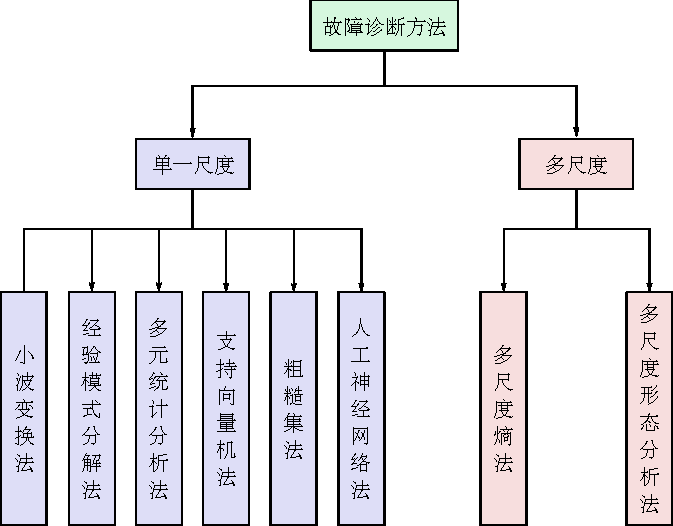
\includegraphics{method_summary}
  \caption{数据驱动的故障诊断方法分类}
  \label{fig:method_summary}
\end{figure}

\subsection{单一尺度的故障诊断方法}

目前大部分数据驱动的故障诊断方法都是基于单一尺度特征的。这一类方法有基于
信号处理的小波变换法、经验模式分解法等;基于多元统计分析的方法如偏最小二
乘法、主元分析法、指定元分析法、独立元分析法、核主元分析法等;基于支持向
量机的方法;基于粗糙集的方法;基于人工神经网络的方法等。

1)小波变换法

小波变换(Wavelet Transform)是指以一种有限长、快速衰减、被称为母小波的振
荡波形为基函数,通过平移和缩放来表示输入信号的过程。从提出到现在,小波变
换在理论和应用上都取得了巨大的发展,包括连续小波变换、离散小波变换、小波包
变换以及近些年提出的第二代小波变换等,在各类系统的故障诊断中都得到了大量的应用。

文献~\inlinecite{zuo2005feature}将信号$x(t)$的连续小波变换(Continuous Wavelet
Transform, CWT)的小波系数作为初始特征,结合主元分析和指定元分析方法实现
了齿轮箱的故障诊断。文献~\inlinecite{zhu2009synchronous}将小波系数映射到
极坐标系中,以增强由齿轮箱和轴承故障引起的周期性瞬变特征。文献~\inlinecite{meltzer2004fault}
同样使用极坐标系下的小波系数,提高了在非平稳转速下运行的故障齿轮的检测能
力。文献~\inlinecite{nagaraju2009application}使用3维CWT提取信号在时频两域
的特征,并结合相位角信息,提升了转子裂纹的检测能力。文献~\inlinecite{rafiee2009use}
将小波系数的自相关函数近似为简单的正弦函数,并应用到齿轮箱故障诊断的特征
提取过程中。文献~\inlinecite{peter2004machine}基于遗传算法设计的精确小波
分析过程进一步优化了小波系数,并应用于电动泵的故障诊断中。

离散小波变换(Discrete Wavelet Transform, DWT)的多分辨率分析能力使得它非
常适合从采集自旋转机器上的非平稳信号中提取故障相关的信息。文献\inlinecite{kim2007comparative}
对转子系统的损伤检测进行了比较研究,发现在包括短时傅立叶变换(Short Time
Fourier Transform, STFT),Wigner-Ville分布(Wigner-Ville Distribution, WVD)
和DWT在内的各种时频技术中,从加速和减速过程收集的振动信号中提取与裂纹状态
有关的特征,DWT是其中最有效的方法。文献~\inlinecite{omar2012dynamic}设计了
一种动态的窗口小波多分辨率分析方法,用于在嘈杂的环境中检测和定位齿轮缺陷。
文献~\inlinecite{djebala2008detection}在优化了小波多分辨率分析过程的基础
上,使用峰度作为优化和评估标准,完成了对轴承的故障检测。在许多研究中已经
广泛采用基于DWT的去噪方法,来消除背景噪声并增强测量信号中包含的故障相关信
息。文献~\inlinecite{li2011virtual}设计了一个基于DWT、自回归(Autoregressive,
AR)模型和主成分分析的齿轮故障诊断方法,其中DWT的作用就是对原始振动信号进
行去噪。

小波包变换(Wavelet Packet Transform, WPT)具有更强的高频信号分解能力,这
使它成为检测和区分具有高频特性的瞬态分量的最佳工具之一。在文献~\inlinecite{gao2006non}
中,对比研究了WPT和其他时频分析技术用于非平稳信号处理的效果,发现WPT能够识
别轴承振动信号内由于缺陷引发的瞬态分量,以及与缺陷增长的相变相关的频移。WPT
也常被用作预处理器将原始信号分解成窄带信号,以提高希尔伯特 - 黄变换(Hilbert–Huang
Transform)的性能~\cite{peng2005comparison}。文献~\inlinecite{tian2010hybrid}
使用WPT作为预处理工具来减少WVD中通常存在的交叉干扰,增强了WVD在轴承故障诊
断中的能力。此外,从WPT的小波系数中提取的某些特征也被广泛用于直接表征机器
的故障状态。文献~\inlinecite{zarei2007bearing}将WPT应用于感应电动机定子电
流信号,并且提取子频带能量作为故障指标来检测轴承故障。文献~\inlinecite{li2008wavelet}
设计了一种基于小波的高阶统计方法用于滚动轴承的故障诊断,并且以WPT和DWT的
小波系数中提取的峰值作为损伤检测和分类的度量。

由于计算速度快,易于实施,近些年来将第二代小波变换(Second Generation
Wavelet Transform, SGWT)应用于旋转机械故障诊断的应用越来
越多。文献~\inlinecite{chen2007vibration}使用SGWT从水力电机的振动信号中提
取特征,对不同的活塞故障状态进行分类。文献~\inlinecite{he2009principle}通
过将SGWT应用于从数控机床的铣削过程测量的声发射信号来检测铣刀破损。文献~\inlinecite{bao2009anti}
为解决故障特征提取中的频率混叠问题,使用抗锯齿SGWT对信号进行了变换,
从而达到了较高的故障分类精度。文献~\inlinecite{hongkai2006gearbox}使用自
适应冗余SGWT分析了具有磨损故障的齿轮箱的振动信号,并从复杂背景中提取了脉
冲分量。同样,SGWT也经常被用来对信号进行去噪处理。在自适应SGWT的基础上,
文献~\inlinecite{li2012adaptive}设计了一种自适应形态梯度提升小波变换,以
增强由轴承缺陷引起的脉冲特征,同时抑制原始信号中包含的噪声。文献~\inlinecite{li2011mechanical}
提出了一种基于冗余非线性SGWT的去噪方法来去除机械故障信号中包含的噪声。

2)经验模式分解法

经验模式分解(Empirical Mode Decomposition, EMD)是黄锷(N. E. Huang)等人于1998年提出的一种自适应信号时频处理
方法~\cite{huang1998empirical}。EMD根据数据自身的时间尺度特征进行信号分解,
并不需要预先指定基函数。这与分别建立在预先指定的谐波基函数和小波基函数上的
傅里叶变换与小波变换有本质的区别。这使得EMD在理论上可以应用于任何类型的信
号分解,因此尤其在处理非平稳和非线性的数据时,EMD具有非常明显的优势,得出
的结果具有很高的信噪比。信号经过EMD分解得到的有限个分量称为本征模函数(Intrinsic
Mode Function,IMF),各IMF分量包含了原始信号在不同时间尺度的局部特征信号。
与STFT、小波变换等方法相比,由于EMD的基函数是由数据本身分解得到,并且分解
过程是基于信号序列时间尺度的局部特性进行的,因此EMD是直观、后验和自适应的。

文献~\inlinecite{gaoqiang2007empirical}使用EMD分解将带有局部损伤的滚动轴
承所产生的高频调幅信号成分作为IMF分离出来,然后通过希尔伯特变换(Hilbert
Transform)得到其包络信号和包络谱,进而提取出滚动轴承故障的特征频率并完成
故障诊断。文献~\inlinecite{xu2009life}采用EMD分析轴承加速寿命试验的振动信
号,并研究了轴承寿命周期的演变趋势。文献~\inlinecite{junsheng2007application}
提出了基于EMD的能量算子解调方法,并用于轴承的故障诊断中。文献~\inlinecite{fan2008machine}
利用IMF的振幅加速能量来表示轴承和齿轮的故障特征。

EMD虽然有较好的处理非线性和非平稳信号的能力,但是同时也存在一定的问题,如
缺乏理论基础、端点效应、筛选停止标准、极值插值、模式混叠等。文献~\inlinecite{rato2008hht, chen2012signal, wu2009ensemble}
对此进行了详细的讨论。此外,也有一些针对此类问题的改进方法被提出。例如文献~\inlinecite{wu2009ensemble}
提出的集成经验模式分解(Ensemble Empirical Mode Decomposition, EEMD)方法,
通过在信号中增加噪声,解决了原始EMD方法模式混叠的问题。文献~\inlinecite{ai2009condition}
提出了一种基于EEMD和包络谱的方法,并可靠地诊断出了轴承的局部缺陷。文献~\inlinecite{zhouzhi2013eemd}
在使用EEMD对信号进行分解的基础上,使用互相关系数进行自适应重构从而突出故障
特征信号,并且使用谱峭度(Spectrum Kurtosis)确定带通滤波器的中心频率及带
宽,最后在滤波的结果上进行了能量算子解调谱分析,从而完成了滚动轴承的故障诊
断过程。文献~\inlinecite{dong2009sifting}提高了EMD筛选过程的效率,并实现了
轴承的内圈故障检测。

3)多元统计分析法

多元统计分析方法主要用于分析拥有多个变量的样本之间的关联性,或是厘清数
据的结构。基于多元统计分析的故障诊断方法的基本思想是:使用多元投影过程
对多变量样本空间进行分解,在子空间中构造反映空间变换的统计量,以计算出
的统计量作为指标检测设备运行过程中的故障状态,基于多元统计分析的故障诊
断方法主要有偏最小二乘法、主元分析法、指定元分析法、独立元分析法、核主
元分析法等。

偏最小二乘(Partial Least Squares, PLS)是一种基本的多元统计方法,广泛
用于故障检测和诊断领域。通过使用离线训练的模型和在线的过程数据测量,可
以实现工业过程关键性能指标的在线预测。PLS能够发现输入输出数据中包含的关
联信息,从而检测过程输入中发生的故障~\cite{li2010geometric, zhang2010decentralized, muradore2012pls}。
文献~\inlinecite{zhou2010total}基于PLS提出了一种被称为全投影(Total Projection
to Latent Structures, TPLS)的方法来处理标准PLS中存在的倾斜分解问题,并
将这种方法应用在过程监控与故障诊断中。文献~\inlinecite{yin2011study}提出
了一种改进的PLS方法,与其他现有的基于PLS的过程监控与故障诊断方法相比,能
够在提供更好性能的同时也节省计算成本。

主元分析(Principal Component Analysis, PCA)的提出最初是为了降低大型相
关数据集的维数,同时仍然保留原始数据集中的大部分信息~\cite{abdi2010principal}。
由于其简单的形式和处理大量数据的能力,PCA已经广泛应用于许多计算领域,如
图像分析、特征提取、模式识别、数据压缩和时间序列预测等。此外,PCA在过程
监控和故障诊断领域的应用也得到了极大的发展~\cite{joe2003statistical, gertler2004pca, choqueuse2012diagnosis}。

为了实现薄板夹具多重组合故障的检测,文献~\inlinecite{liu2005assembly}提
出了指定元分析(Designated Component Analysis, DCA)方法。DCA首先根据零
件的几何特性和传感器的布局等知识定义一组相互正交的向量来表示故障模式,
然后在测量的数据上计算它们的统计学显着性,这相当于将组合故障分解到了一
组预定义的相互正交的故障模式上。最后利用这些故障模式的显著性实现多重组合
故障的检测。

作为另一种常见的多元统计方法,独立元分析(Independent Component Analysis,
ICA)通过将独立元从过程测量中分离出来,解决了盲源分离问题~\cite{hyvarinen2004independent}。
ICA近些年来也被很多学者应用于故障检测的目的,特别是针对那些输入输出不是
高斯分布的故障诊断问题~\cite{kano2003monitoring, lee2004statistical}。

PCA实际上是将多元数据样本从一个空间线性映射到另一个空间的方法,难以分析
具有非线性特征的数据,因此出现了基于核主元分析(Kernel Principal Component Analysis, KPCA)
的故障诊断方法。文献~\inlinecite{lee2004nonlinear}使用KPCA进行特征提取并
结合统计图的方法完成生物废水处理过程中故障的检测。文献~\inlinecite{sun2007evolving}
基于KPCA和一种改进的进化算法提出了进化核主元分析(Evolving Kernel Principal
Component Analysis, EKPCA)方法用于旋转机器的故障诊断。文献~\inlinecite{he2007subspace}
在信号的频域特征以及经过WPT预处理的信号时域特征的基础上,利用KPCA提取非
线性特征,并通过构造子空间的方法实现齿轮箱的故障诊断。

4)支持向量机法

支持向量机(Support Vector Machine, SVM)是20世纪90年代中期发展起来的机
器学习方法,尤其适合处理少量非线性高维数据样本的分类或回归问题,因此也广
泛应用于故障诊断领域~\cite{huqiao2006improved}。

文献~\inlinecite{aydmj1999pump}分别使用功率谱、包络谱、自回归建模、Music
谱和经典谱提取特征,并使用SVM对提取的特征分类,实现了小型潜水泵的故障检
测。文中对比了这几类特征提取方法与SVM结合做故障诊断的效果,并提出了支持
向量数据描述(Support Vector Data Description, SVDD)方法来寻找包含所有
目标数据的最小球体。

文献~\inlinecite{jack2002fault}使用SVM和人工神经网络对滚动轴承的钢球故障、
外圈故障、滚动体故障和壳体故障四种故障状况进行检测。文中基于矩和累积量来
定义和计算统计学特征,并使用遗传算法(Genetic Algorithm, GA)来选择最佳
特征。此外,也有其他一些文献以时间序列的矩、累积量等高阶统计量作为特征训
练SVM分类模型,用于故障诊断问题当中~\cite{ren2005application, sugumaran2007feature, hu2007fault, yang2005cavitation}。

文献~\inlinecite{shuang2007bearing, chang2008fault}使用PCA从原始数据中提
取特征并在此基础上训练SVM分类器,分别实现了滚动轴承和矿井提升机的故障诊断。
此外,也有一些使用其他多元统计方法提取特征,并结合SVM实现故障诊断的方法,
如文献~\inlinecite{widodo2007combination, widodo2005fault}使用ICA和SVM结
合的方法对感应电机的故障进行了诊断,文献~\inlinecite{ni2011adaptive}结合
KPCA和SVM提出了一种自适应的故障诊断方法并将其用于检测高压断路器的故障。

文献~\inlinecite{yang2007fault}提出了一种基于EMD和SVM的故障诊断方法,并将
其应用于滚动轴承的故障诊断中。在使用EMD算法将原始信号分解为多个IMF之后,
计算包括主要故障信息的一些IMF的包络谱。然后将每个IMF包络谱中不同故障特征
频率处的振幅比定义为特征振幅比。最后,以特征振幅比作为SVM分类器的特征向
量,实现滚动轴承工作状态和故障模式的检测。

在故障诊断方法中,SVM通常是作为特征分类器完成系统状态或故障模式的分类,
故障特征的获取过程依赖于前面介绍的一些信号处理、统计分析的方法,因此SVM
方法一般是和其他故障诊断方法结合使用的。

5)粗糙集法

Pawlak在1982年首先提出粗糙集理论(Rough Set Theory, RST)。RST是一种非常
有效的多属性分类方法,其最大的优势在于能够对不精确、不确定或不完整的数据
进行分类。经过几十年的发展,RST已经被广泛应用于许多领域,如医疗诊断、股
票市场预测、工业系统故障诊断、银行决策系统等。

文献~\inlinecite{tay2003fault}以信号的频域波形复杂度、频谱中心频率、信号
时域复杂度、信号非周期复杂度、方差、峰度这6个特征作为属性,将它们离散化
之后的结果用于训练RST,并对多缸柴油发动机的阀门故障进行了识别,该方法克
服了常规故障诊断方法只能识别一种故障的缺点。文献~\inlinecite{wu2010power}
基于RST和SVM提出了一种变压器故障位置的检测方法。文中使用RST将油料数据和
电气数据的结果进行组合和约简,建立故障和信息的映射,然后通过SVM对映射进
行分类,诊断变压器的故障位置。

RST要求输入数据的属性必须是离散的,因此在使用RST学习决策规则之前,必须对
输入的数据做离散化处理,这限制了RST在很多问题中的应用。因此能够处理连续
取值数据的模糊RST更常用于故障诊断问题中。文献~\inlinecite{hao2006improved}
使用数据库知识发现(Knowledge Discovery in Database, KDD)技术挖掘数据中
的聚类信息,确定属性集合和模糊取值并约简模糊规则,最后利用模糊RST学习变
压器中的早期故障模式。

6)人工神经网络法

近些年来,人工神经网络(Artificial Neural Network, ANN)在高度复杂系统建
模方面取得了巨大的成功。由于ANN在理论上可以表示任何非线性模型,而不用了解
其实际的内部结构,因此被广泛用于故障诊断领域进行故障特征分类。与SVM类似,
ANN通常也是和其他一些信号时频特征提取方法或统计特征提取方法结合使用来完成
故障诊断的。

文献~\inlinecite{sorsa1991neural}以14个带有噪声的测量信号作为ANN的输入,
10个故障类型作为ANN的输出,并使用双曲正切为激活函数的多层感知网络结构来检
测热交换器 - 连续搅拌釜反应器系统中的故障。文献~\inlinecite{li2000neural}
将滚动轴承的频率特征作为ANN的输入,用于电机轴承系统中轴承缺陷类型的诊断。
文献~\inlinecite{paya1997artificial}通过小波变换对驱动线获得的实时振动信
号进行预处理,并作为ANN的输入,完成了驱动线的单一轴承故障、单一齿轮故障
以及两者同时发生的多重组合故障的检测。文献~\inlinecite{yu2006roller}提出
了一种基于EMD能量熵和ANN的滚动轴承故障诊断方法。该方法从EDM分解得到的IMF
分量中提取能量特征,并作为ANN的输入,实现了轴承内圈故障和外圈故障的检测。

文献~\inlinecite{goode1994hybrid}提出了一种基于混合模糊ANN的故障诊断方法,
该方法利用模糊规则和模糊隶属度函数在分析启发式知识上的优势,结合ANN强大的
非线性模型拟合能力,完成了对单相感应电机系统轴承早期故障的检测。文献~\inlinecite{kang2006certainty}
提出了一种基于模糊神经网络(Fuzzy Neural Network, FNN)的故障诊断方法,对
振动信号中提取的频率特征进行分类,从而对电机轴承系统进行故障检测,获得了
较好的诊断结果。文献~\inlinecite{dong2008rough}提出了一种基于RST和模糊小波
神经网络(Fuzzy Wavelet Neural Network, FWNN)的故障诊断方法。该方法首先使
用RST来挖掘数据中的潜在规则,当置信度符合预先设定的标准时,直接使用这些规
则对电力变压器的故障状态进行推断;对于置信度不符合预设标准的情况,使用7个
具有不同隐层个数、不同学习率等训练相关参数的子FWNN分别进行特征分类,最后使
用最小二乘加权融合算法对这7个子FWNN的输出进行融合,实现了电力变压器系统中
热故障、低能量放电故障以及高能量放电故障的诊断。

\subsection{多尺度的故障诊断方法}
\label{subsection:multiscale_methods}

\subsubsection{多尺度熵算法}

时间序列的复杂度可以通过多种方法进行研究,例如近似熵~\cite{valenza2014inhomogeneous}
和样本熵~\cite{yentes2013appropriate}。然而,这些方法并没有考虑广泛存在于实际
物理系统中的多种时间尺度。因此,Costa等人于2002年提出了多尺度熵(MSE)方法
,通过计算不同尺度下序列的样本熵,来表示时间序列在不同尺度下的复杂性~\cite{costa2002multiscale}。

由于MSE的计算依赖于样本熵,因此在介绍MSE的计算方法之前,我们先来介绍样本熵。
对于一个长度为$N$的原始时间序列$x=\{x_1, x_2, ..., x_N\}$,记$x(i)=\{x_i, x_{i+1}, ..., x_{i+m-1}\}$
为原始序列$x$的第$i$个长度为$m$的子序列。样本熵定义为一个条件概率,它量化长
度为$m$的子序列与另一个相同长度的子序列相等(在r的误差容忍范围内)时,将它
们的长度增加为$m+1$后仍然相等的概率。我们将$m$称为嵌入维数。两个子序列之间
距离定义为对应元素差值绝对值的最大值。例如,序列$x(i)$与序列$x(j)$之间的距
离$d_{ij}$定义为~(\ref{equ:chap1:l1_norm})式。
\begin{equation}
  \label{equ:chap1:l1_norm}
  \begin{aligned}
    d_{ij} = & d(x(i), x(j)) \\
    = & \max_{k=0}^{m-1}|x(i+k)-x(j+k)|
  \end{aligned}
\end{equation}

将两个长度为$m$的子序列相等(在r的误差容忍范围内)的概率记作$B^m(r)$。那么
$B^m(r)$可以如下计算:对每个$i$,计算$x(i)$与其余子序列$x(j)(j=1,2,...,N-m; j\neq i)$
的距离$d_{ij}$,并统计$d_{ij}$小于$r$的平均个数,如~(\ref{equ:chap1:bmr})式所
示。
\begin{equation}
  \label{equ:chap1:bmr}
  B^m(r)=\frac{1}{(N-m)(N-m-1)}\sum_{i\neq j}\theta(r-d_{ij})
\end{equation}

其中$\theta(x)$是单位阶跃函数:
\begin{equation}
  \label{equ:chap1:step_func}
  \theta(x) = \left\{
  \begin{aligned}
    1 &, x > 0 \\
    0 &, x \leq 0
  \end{aligned}
  \right.
\end{equation}

样本熵可以定义为~(\ref{equ:chap1:sample_entropy})式。
\begin{equation}
  \label{equ:chap1:sample_entropy}
  \text{SampEn}(m, r) = \lim_{N\to\infty}-\ln\frac{B^{m+1}(r)}{B^m(r)}
\end{equation}

在$N$为有限值时,~(\ref{equ:chap1:sample_entropy})式可以写成~(\ref{equ:chap1:sample_entropy_finite})
式。
\begin{equation}
  \label{equ:chap1:sample_entropy_finite}
  \text{SampEn}(m, r, N) = -\ln\frac{B^{m+1}(r)}{B^m(r)}
\end{equation}

根据Trunkvalterova等人~\cite{trunkvalterova2008reduced}的研究,嵌入维度$m$
通常取2,误差容忍度$r$通常取原始时间序列标准差的0.15倍。正常和周期信号的理
论样本熵为0,而不相关的随机信号具有最大样本熵(该值取决于信号长度)。

MSE算法由以下两个步骤组成~\cite{costa2002multiscale, costa2005multiscale}:

1)通过一系列粗粒化(coarse grained)过程,计算原始时间序列在不同尺度上的
一组表示序列。在尺度为$\tau$的粗粒化过程中,将给定时间序列的每个长度为$\tau$
的连续不重叠区间内的数据点进行平均,所得的结果作为尺度$\tau$下的粗粒化表示
序列。例如,对于一个长度为$N$的离散信号$\{x_1,...,x_i,...,x_N\}$,原始时间
序列在尺度$\tau$下的粗粒化表示序列$\{y^{(\tau)}\}$的计算方式如~(\ref{equ:chap1:coarse_grained})
式所示。
\begin{equation}
  \label{equ:chap1:coarse_grained}
  y^{(\tau)} = \frac{1}{\tau}\sum_{i=(j-1)\tau + 1}^{j\tau}x_i , 1\leq j\leq N/\tau
\end{equation}

尺度为$\tau=1$时,粗粒化表示序列$y^{(1)}$对应原始信号。序列$y^{(\tau)}$的
长度为$N/\tau$。

2)计算每个粗粒化表示序列$y^{(\tau)}$的样本熵,得到由$\tau$个样本熵值构成的
序列,即为MSE的结果。对每个粗粒化表示序列求样本熵时,使用相同的误差容忍度$r$。

从提出以来,MSE已经成为量化信号复杂度的普遍方法。由于MSE对非线性、非平稳
序列有良好的处理能力,而且具有多尺度特征的提取能力,因此已经成功应用于很
多研究领域。在故障诊断领域也得到了非常广泛的应用。

文献~\inlinecite{zhang2010bearing}计算了20个尺度上的MSE,并在此基础上构造
了最大值、最小值、算术平均值、几何平均值以及标准差这5个统计值作为特征,结
合自适应模糊神经推断系统(Adaptive Neuro-fuzzy Inference System, ANFIS)
实现了对滚动轴承的故障诊断。文献~\inlinecite{zhengjinde2012mse}使用MSE算法
对滚动轴承的振动信号进行特征提取,并比较了MSE算法相对于单一尺度下的样本熵
算法的优势,最后使用支持向量机作为分类器,完成了滚动轴承故障类型的识别。文
献~\inlinecite{liu2014fault}使用局部平均分解(Local Mean Decomposition, LMD)
将滚动轴承的非平稳振动信号分解成多个项的乘积,并计算各乘积项的MSE作为特征,
实现了多种类型的故障状态的识别。文献~\inlinecite{zhanglong2014mse}基于时间
序列的MSE的偏度(Skewness)和均值构造了一个故障程度定量描述指标——多尺度熵
偏均值(Partial Mean of Multiscale Entropy, PMME),实现了轴承故障程度的评
估,并且能够跟踪故障发展的趋势。

在MSE的基础上,也有很多研究人员针对其存在的一些问题提出了相应的改进算法。
文献~\inlinecite{humeau2015multiscale}对原始的MSE算法以及很多不同的改进算
法进行了综述。例如文献~\inlinecite{xie2008measuring}提出,MSE算法所依赖的
样本熵的计算过程中用到了阶跃函数,从而引入了不连续因素,因此使用连续的Sigmoid
函数来替代阶跃函数,提出了多尺度模糊熵(Multiscale Fuzzy Entropy, MFE)算
法。

文献~\inlinecite{zhengjinde2014mfe}使用多尺度模糊熵对滚动轴承的振动信号
进行特征提取,并使用SVM作为分类器,实现了滚动轴承外圈、内圈和钢球3种故障
状态的识别。文献~\inlinecite{zhengjinde2016cmfe}针对MSE粗粒化方式的不足,
提出了复合多尺度模糊熵(Composite Multiscale Fuzzy Entropy, CMFE)算法来
度量时间序列的自相似性和复杂性。CMFE综合了序列在同一尺度下多种粗粒化方式
的结果,获得更加稳定和一致的特征。在此基础上,结合Fisher得分进行特征选择
并通过SVM进行分类,完成了对滚动轴承的故障诊断过程。

\subsubsection{多尺度形态分析}

数学形态学(Mathematical Morphology, MM)~\cite{haralick1987image}是一种
非线性分析方法,最初是为图像处理而设计的,后来在信号分析等领域也得到了广
泛的应用。通过对原始信号进行形态分解~\cite{pitas1990morphological},复杂
信号可以从背景中分离出来,并分解为保留了原始信号形态特征的多种分量。信号
形态处理的基本思路是通过一些形态变换来改变信号的形状。基本的形态变换算子
有扩张、腐蚀、开、闭运算。

令$f(n), n={0, 1, ..., N-1}$表示一个一维信号,$g(n), n={0, 1, ..., M-1}$
表示一个结构元素(Structuring Element, SE),腐蚀和扩张算子可以定义为~(\ref{equ:chap1:erosion_dilation})
式。
\begin{equation}
  \label{equ:chap1:erosion_dilation}
  \begin{aligned}
    (f\ominus g)(n) = & \min_{m=0}^{M-1}\left[f(n+m)-g(m)\right] \\
    (f\oplus g)(n) = & \max_{m=0}^{M-1}\left[f(n-m)+g(m)\right]
  \end{aligned}
\end{equation}

其中$\ominus$表示腐蚀运算,$\oplus$表示扩张运算。基于这两种运算,另外两
种形态变换算子开、闭运算可以由~(\ref{equ:chap1:opening_closing})式定义。
\begin{equation}
  \label{equ:chap1:opening_closing}
  \begin{aligned}
    (f\circ g)(n) = & (f\ominus g\oplus g)(n) \\
    (f\bullet g)(n) = & (f\oplus g\ominus g)(n)
  \end{aligned}
\end{equation}

其中$\circ$表示开运算,$\bullet$表示闭运算。表~\ref{tab:morphological_operator_effect}
列出了四种基本形态运算对信号脉冲的影响。
\begin{table}[htb]
  \centering
  \begin{minipage}[t]{0.6\linewidth}
  \caption{四种基本形态运算对信号脉冲的影响}
  \label{tab:morphological_operator_effect}
    \begin{tabularx}{\linewidth}{XXX}
      \toprule[1.5pt]
      形态运算 & 正脉冲 & 负脉冲 \\\midrule[1pt]
      腐蚀 & 抑制 & 平滑 \\
      扩张 & 平滑 & 抑制 \\
      开运算 & 抑制 & 保留 \\
      闭运算 & 保留 & 抑制 \\
      \bottomrule[1.5pt]
    \end{tabularx}
  \end{minipage}
\end{table}

此外,还有其他一些由这些运算组合而成的形态运算,例如比较常用的平均算子AVG
和梯度算子DIF,如~(\ref{equ:chap1:average_difference})式所示。
\begin{equation}
  \label{equ:chap1:average_difference}
  \begin{aligned}
    AVG(f) = & (f\bullet g + f\circ g)/2 \\
    DIF(f) = & f\bullet g - f\circ g 
  \end{aligned}
\end{equation}

在实际应用中,通常根据信号处理的不同场景选择或组合使用合适的形态运算。
SE是形态分析的另一个关键部分。通常,只有当所关心的信号成分的尺度和形
状与SE的尺度和形状匹配时,才能在经过形态运算后保留下来。因此,应该根
据待分析的信号来选择SE的形状、长度和高度(振幅)。SE的形状可以从规则
到不规则的曲线变化,例如水平线、三角和半圆等,如图~\ref{fig:se_shape}
所示。
\begin{figure}[ht]
  \centering
  \subcaptionbox{呈水平状的SE\label{fig:se_shape_flat}}
  {
\includegraphics[width=3cm]{se_flat}}
  \hspace{4em}
  \subcaptionbox{呈三角状的SE\label{fig:se_shape_triangular}}
  {
\includegraphics[width=3cm]{se_triangular}}
  \hspace{4em}
  \subcaptionbox{呈半圆状的SE\label{fig:se_shape_semicircular}}
  {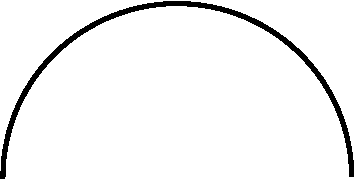
\includegraphics[width=3cm]{se_semicircular}}
  \caption{不同形状的SE}
  \label{fig:se_shape}
\end{figure}

SE的尺度,包括长度和高度对于一维信号的形态分析也很重要。传统的形态分
析是在单一尺度下进行的,其中SE是根据先验知识来设定的。然而这些先验知
识并不是在任何情况下都适用,而且很多问题中我们很难获取到这些先验知识。
因此,为了从信号中提取不同尺度的形态特征,需要进行多尺度形态分析。多
尺度形态分析是使用多种尺度的一组SE,分别对原始信号进行形态分析,从而
获得多种尺度下特征的过程。

文献~\inlinecite{haorujiang2008mmf}使用形态开运算对滚动轴承振动信号
进行多尺度形态分解,并计算不同尺度下的形态谱,然后在此基础上计算不同
尺度下信号的形态谱熵值,进而以此为特征完成了不同故障类型的定量区分。
文献~\inlinecite{wangbing2013mmf}使用多尺度形态分析将电机滚动轴承的
振动信号分解到多个尺度上,并在此基础上计算能谱熵和奇异谱熵作为特征,
结合灰色关联分析,完成了对电机轴承退化状态的评估。文献~\inlinecite{libing2011adaptive, li2011weighted}
使用梯度形态算子和水平状SE对滚动轴承的振动信号进行了多尺度形态分解,
并且定义了一种自适应的权值计算方法,对分解得到的各尺度下的信号进行
加权,使得小尺度下分解得到的信号具有较小的权重,大尺度下分解得到的
信号具有较大的权重,从而在保留原始信号细节的同时有效地抑制了噪声。
从实验结果可以看出这种方法能够有效地从故障轴承的振动信号中提取出特
征冲击信号。文献~\inlinecite{tangguiji2015adaptive}使用Top-Hat形态
算子对滚动轴承的振动信号进行多尺度形态分析,并在此基础上通过计算特
征幅值能量比(Feature Amplitude Energy Radio, FAER)来自适应地选择
最佳尺度,成功地应用于轴承的故障增强检测当中。

\section{论文组织结构}

本文的组织结构框架如图~\ref{fig:overall_structure}所示。本文主要研
究了基于深度神经网络的多尺度故障诊断方法。首先在第一章对目前常见的
单一尺度和多尺度故障诊断方法进行了综述;第二章基于传统的机器学习方
法设计了一种单一尺度的故障诊断模型,对下采样操作用于信号特征提取的
效果进行了验证;第三章基于深度神经网络设计了一种单一尺度的故障诊断
方法,实现了信号特征的逐层提取和抽象过程,验证了深度神经网络用于信
号特征提取和故障模式分类的强大能力;在第二章和第三章的基础上,第四
章设计了一种基于深度神经网络的多尺度故障诊断方法,实现了多种尺度下
特征的自动提取与融合。下面我们对每一章的内容做简要介绍。
\begin{figure}[ht]
  \centering
  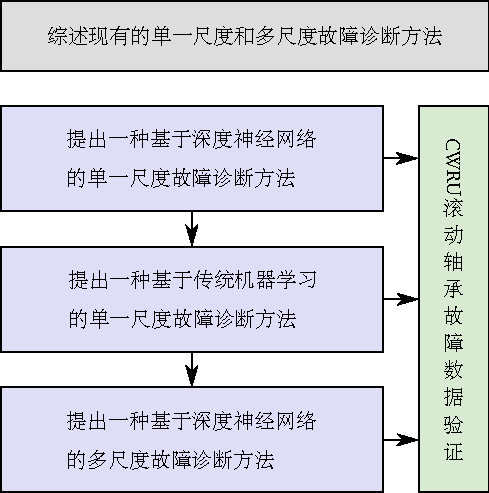
\includegraphics{overall_structure}
  \caption{论文组织结构框架图}
  \label{fig:overall_structure}
\end{figure}

第~\ref{cha:intro}章是论文的引言。首先简单介绍了故障诊断技术的背景
和意义,以及故障诊断的概念和需要完成的任务;接下来分析了数据驱动的
故障诊断方法相对于传统的基于模型的故障诊断方法的优势,并且根据能否
有效利用输入数据在多个尺度上的特征将数据驱动的方法分为单一尺度的方
法和多尺度的方法;最后分别介绍了这两类方法的研究现状。

第~\ref{cha:chapter2}章介绍了基于下采样操作和级联SVM提出的一种单一
尺度的故障诊断方法。这一章是本文提出的三种故障诊断方法的基础,在简
要地阐述了RDFT和SVM的原理之后,介绍了本文三种故障诊断方法中都使用
的数据预处理过程;接下来介绍了本章使用单层下采样进行特征提取和压缩
的过程,以及设计的级联SVM分类模型;然后简单地介绍了本文实验中所用
的CWRU滚动轴承故障数据集,最后在CWRU数据集上进行实验验证时,我们考
察了特征提取阶段使用的下采样操作的核宽度对最终诊断精度的影响,我们
发现核宽度过大或过小均会导致诊断精度的下降,这是只用单层下采样进行
特征提取和压缩的局限。此外,本章还对最优核宽度下提取的特征进行了可
视化,给出了诊断精度和混淆矩阵并进行了分析。

第~\ref{cha:chapter3}章介绍了基于卷积神经网络(CNN)提出的一种单一
尺度的故障诊断方法。由于第~\ref{cha:chapter2}章中提出的基于单层下
采样的故障诊断方法有一定的局限性,因此我们考虑采用多层下采样操作逐
层提取和抽象特征的结构,而CNN正是为这样的任务设计的。本章在简要地
阐述了人工神经网络(ANN)和CNN的原理之后,介绍了本章中的故障诊断方
法通过多层卷积和下采样操作完成特征提取并通过全连接层完成特征分类的
过程;最后在CWRU数据集上进行了实验验证,可以发现本章基于CNN的故障
诊断方法在诊断精度上明显优于第二章基于单层下采样的方法。

第~\ref{cha:chapter4}章介绍了基于CNN提出的一种多尺度故障诊断方法。
根据~\ref{subsection:multiscale_methods}节的介绍,实际物理系统由于
多种组成部件以及所处环境间的相互作用,通常带有多种尺度的特征。此外,
从第~\ref{cha:chapter2}章的实验分析可知,采样程度低时对应的大尺度
特征往往带有更多的细节特征,而采样程度高时对应的小尺度特征往往带有
更多的整体特征。而第~\ref{cha:chapter3}章中提出的基于CNN的故障诊断
方法中,由于网络中多个下采样层是顺序连接的,因此网络中的特征的尺度
是不断减小的,无法达到多种尺度下特征的融合效果。因此本章在第~\ref{cha:chapter2}、~\ref{cha:chapter3}
章的方法的基础上,提出了一种基于CNN的递归式网络
结构,能够很好地融合多种尺度下输入信号的特征,在CWRU上的实验结果证
明,本章设计的故障诊断方法比单一尺度下的方法更加有效,能够达到更高
的诊断精度。

第~\ref{cha:summary}章总结了论文的工作,并且展望了本课题进一步的研
究方向。
